\documentclass[10pt,twocolumn,letterpaper]{article}

\usepackage{cvpr}
\usepackage{times}
\usepackage{epsfig}
\usepackage{graphicx}
\usepackage{amsmath}
\usepackage{amssymb}

\graphicspath{ {./} }

% Include other packages here, before hyperref.

% If you comment hyperref and then uncomment it, you should delete
% egpaper.aux before re-running latex.  (Or just hit 'q' on the first latex
% run, let it finish, and you should be clear).
\usepackage[breaklinks=true,bookmarks=false]{hyperref}

\cvprfinalcopy

% Pages are numbered in submission mode, and unnumbered in camera-ready
%\ifcvprfinal\pagestyle{empty}\fi
\setcounter{page}{1}
\begin{document}

%%%%%%%%% TITLE
\title{Learning to Feel: Training a CNN to recognize emotion}

\author{Paul Carroll, Connor Smith, Frank Zheng, William Jarrold, Mana Lewis\footnotemark \\
Stanford University\\
{\tt\small \{paulc3, csmith95, fzheng\}@stanford.edu}\\
{\tt\small william.jarrold@gmail.com}\\
{\tt\small mana@chezmana.com}
}

\maketitle
\footnotetext{William and Mana helpfully provided data and links to academic papers. Neither is enrolled in CS231N.}
%\thispagestyle{empty}

%%%%%%%%% ABSTRACT
\begin{abstract}
In the last decade, the development of convolutional neural nets (CNNs) has made it possible for computers to accurately identify the objects in particular images. Now that object recognition is working well, it seems natural to ask the question of whether we can use CNNs to recognize higher-level concepts in photos. In this paper, we apply a modified CNN based on Inception-Resnet to the task of classifying the emotion evoked by particular images. We begin by training our network to classify photos as having positive or negative valence. Next, we set our network a harder challenge, training it to classify photos as belonging to one of eight emotional states (awe, amusement, anger, contentment, fear, disgust, excitement, sadness). We use a dataset of 13K photos collected from social networks. For our valence classification problem, we achieve an accuracy of 91\%. For our eight-fold problem, we achieve a top-one classification accuracy of 69\%.
\end{abstract}

%%%%%%%%% BODY TEXT
\section{Introduction}
In the past few years, with the advent of deep convolutional neural networks, it seems like computers have finally ``solved'' the object classification problem. In the ImageNet Large-Scale Visual Recognition Challenge\cite{imagenet}, algorithms are tasked with identifying which of 1000 possible classes of object is present in a particular image.  Inception-Resnet, a powerful CNN which we will discuss in more detail in the Methods section, has a top-5 classification error of just 3.08\% on the ImageNet test set\cite{inceptionresnet}.

This suggests a question: is it possible to adapt convolutional neural networks to more abstract classification problems? When a human looks at an image, he or she is not merely identifying the objects in that photo. The viewer might also have an emotional reaction. Would it be possible for a deep network to ``learn`` the expected emotional reaction?

This task is more abstract, and correspondingly more difficult, than object recognition. One immediate challenge is that not all humans will agree on which emotions are evoked by which photos. Unlike in the case of object recognition, in which there is an objective source of truth for which objects are or are not contained in a photo, there is no way to ``prove'' that a particular photo evokes excitement or fear or sadness. The only question we can ask is whether a consensus of humans seems to agree on how this photo makes them feel.

It was also not clear when we started this research whether transfer learning from ImageNet would be effective when applied to the task of emotion detection. Transfer learning has successfully been applied to many datasets and classification challenges\cite{transferlearning}. Our classification problem, however, is sufficiently different from object classification that it was not clear whether ImageNet would discover ``useful'' features. It is well understood in the computer vision community that the early layers of a CNN encode edge or color detection. Edge detection is useful if the goal of a neural net is to detect an object class, since every object in a particular class is likely to have a similar shape. But does every photo with negative valence have similar edges? Probably not. Even if we consider the higher-level features which ImageNet learns, such as some internal representation of a cat or a boat, it is easy to imagine a cat or a boat in a photo with negative or positive valence. Part of our research question, then, was to determine if transfer learning from ImageNet would be effective on this task.

We decided to adapt Inception-Resnet to two classification challenges. In the first, we would train it to identify photos as having either positive or negative valence. This simple binary classification challenge would be a good ''sanity check`` for whether emotion detection is possible at all with transfer learning from ImageNet. Next, we would train the classifier to determine which of eight emotional classes each photo belonged to. This would be a harder test for the classifier, since some of the emotional classes were similar to each other: for example, amusement and excitement. We discovered that transfer learning from ImageNet is very effective in the binary classification case, particularly when we augment our training set's data. For the eight-fold classification problem, the classifer's accuracy dropped, but it was still able to identify the correct emotion about two-thirds of the time.

\section{Related Work}
It has long been understood that, in order for machines to be truly intelligent, they will need to be emotionally intelligent. Classifying objects and answering questions is all very well, but a machine which is unable to understand human emotion is less useful to humans than a machine which can.

In 2001, Rosalind W. Picard et al. trained an algorithm to classify eight human emotions\cite{earlyeq}. The input to this algorithm was physiological data--direct measurements of the human subject's vital signs. By using a Fisher projection, the authors were able to achieve 81\% classification accuracy. The methodology of their study was very different from ours, since they were trying to fit physiological data instead of pixel data, but the basic goal of the study was similar: to teach a computer to recognize human emotions.

Later authors suggested approaches for teaching an algorithm to recognize latent emotions in a photo. William Jarrold et al.\cite{methodologyproposed} argued that even though emotional reactions vary among people, there is nevertheless a logic to people's emotions which should be learnable. Because emotions are not completely unpredictable or arbitrary, it should be possible to train an artificial intelligence to anticipate them. Jarrold suggests a methodology for how to evaluate an algorithm's emotional intelligence, but does not provide a procedure for how to build such a model.

In recent years, efforts have begun to build labeled datasets of human emotion for computer vision. In 2017, Kurdi et al. published the OASIS dataset\cite{oasis}, which contains 900 images ranked by human subjects on two dimensions: valence, which is whether the image evokes a negative or positive response, and arousal, which is the intensity of the emotional response. This dataset would be useful for researchers who were interested in learning a regression for valence, but cannot be used for the eight-fold classification problem. Fortunately, another dataset exists for that purpose, published by You et al\cite{ourdata}. We will discuss this dataset further in the next section. You et al. appear to have been the first to train a CNN to classify image data into one of eight emotional categories. On their strongly labeled data, their classifier achieved a top-one accuracy of 58\%. They did not attempt the binary classification problem.

A plethora of examples exist for how transfer learning from ImageNet has solved  classification problems \cite{transferexampleprimary}\cite{transferexample1}\cite{transferexample2}. In particular, Oquab et al.\cite{transferexampleprimary} argue that transfer learning from ImageNet is possible even to datasets with quite different statistical properties from ImageNet, and to datasets which are too small to enable conventional training of deep neural nets. This is highly relevant to our classification challenge, since our dataset is small--just 13,000 images, as opposed to ImageNet's 14 million images. If transfer learning from ImageNet were not possible, it would be highly difficult for us to train a deep neural net over 13k images without overfitting.

\section{Data}
As previously mentioned, our data come from Yun et al\cite{ourdata}. It is worth describing this data in some detail, since the manner in which it was collected and labeled is highly relevant to the classification accuracy which we were able to obtain. They began by querying image search engines for the eight emotions in which they were interested: amusement, anger, awe, contentment, disgust, excitement, fear, and sadness. In this way, they gathered 11,000 images for each emotion. They then used Amazon Mechanical Turk to ask five humans each if they felt the weakly-labeled emotion when looking at each image. For many of these images, zero humans agreed with the proposed label; but for others, a consensus confirmed that the label matched the image.

One observation to make about this dataset is that the methodology of collection doesn't quite fit what we would prefer for a classification problem. In the ideal methodology described by Jarrold et al.\cite{methodologyproposed}, each human participant is asked: Does this photo make you feel angry, awe, amusement...etc.? The question is framed as a multiple-choice. According to You's methodology, a photo which Instagram classifies as ``anger'' will only ever be considered for that category. The human subjects are never asked if the photo would be better classified as ``disgust'' or ``fear.'' This is significant, since, assuming that image search engines haven't solved the problem of machine emotional intelligence, a search engine's decision to label a photo with a particular emotion is probably somewhat arbitrary. The poor quality of these search results is confirmed by the large number of cases in which no humans agreed with the search engine's label. Even if the human subjects agree that a photo returned by the search engine represents ``amusement,'' they are never asked if that photo is an even better representation of ``excitement.'' This flaw in methodology is something that should be corrected in future data-gathering (see the Conclusions section), since it seems likely that it reduces the quality of the labels and therefore the accuracy of the classifier.

\begin{figure}
\centering

\includegraphics[width=0.3\textwidth]{fear-394.png}
\caption{An image classified as ``fear.'' It is possible that this image would have been classified as ``amusement'' if the human raters had been asked whether this photo represents fear or amusement better. Furthermore, it seems flawed that each image is tagged with exactly one emotion. Since a human can certainly feel multiple emotions when presented with an image, a photo should be allowed to have multiple emotional labels.}
\end{figure}

Another question which any user of this data must answer is how many of the human participants need to agree with the weak label before the label is accepted as valid. If three of the five human subjects concur that a photo represents excitement, should that photo be accepted into the training/validation/test sets? What if four of the participants agree? You et al. decided that three was the appropriate cutoff. Because of our skepticism about the quality of the labels, discussed in the previous paragraph, we decided to use four. After we filtered the dataset in this way, we were left with ~13k images.

\begin{figure}
\centering
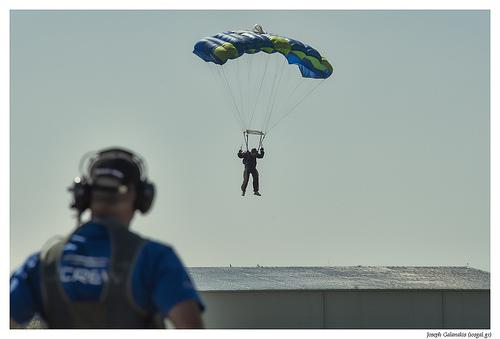
\includegraphics[width=0.5\textwidth]{excitement-1220.png}
\caption{An image classified as ``excitement.'' Once again, it seems possible that, if the human raters had been asked whether this photo represents excitement or fear better, they would have answered fear.}
\end{figure}

One final note is that after the filtering, we were left with a class imbalance. Our largest category, contentment, had 3083 images, while our smallest category, fear, had just 486 images. For more on how we attempted to address this class imbalance, see the Methods section.

\section{Methods}

Our strategy for solving this classification problem was to use transfer learning from ImageNet, rather than training a CNN from scratch. We chose this strategy because our training set of 13k images isn't really sufficient to train a deep neural network. We were bolstered in this decision by the multitude of successful case studies of transfer learning from ImageNet (see the Related Works section).

The particular ImageNet classifier which we decided to use was Inception-Resnet V2, a network released by Google in 2016\cite{inceptionresnet}. The architecture of Inception-Resnet consists of two important pieces: \textit{Inception modules}, or subnetworks which can be stacked on top of each other, and \textit{residual connections}, which create ``shortcuts'' in the model that seem to facilitate backpropagation. We chose Inception-Resnet because of its world-class performance on the ImageNet challenge, scoring a top-five accuracy of 95.2\%.

\begin{figure}
\centering
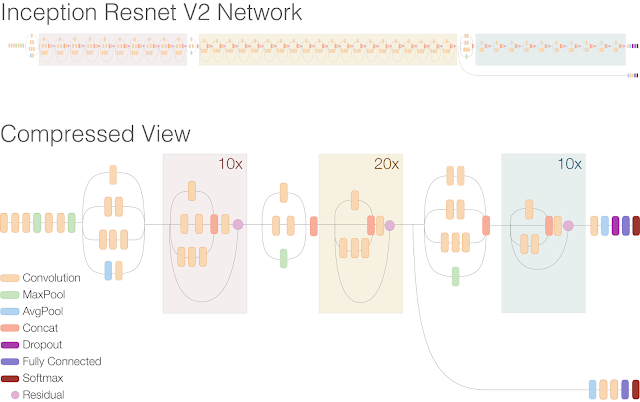
\includegraphics[width=0.5\textwidth]{inception_resnet_architecture.png}
\caption{A schema for the Inception-Resnet architecture.}
\end{figure}

In the final stage of the Inception-Resnet classifier, a feature vector of size 1790 is mapped to the 1000 classes of ImageNet. The scores vector is then converted to class probabilities using a softmax loss function. We replaced these stages with our own logic. The feature vector produced by Inception-Resnet would be passed to our own subnetwork to produce either two scores, in the case of the binary classifier, or eight scores, in the case of the eight-fold classifier. Finally, we would use a softmax loss function to convert these scores into normalized ``probabilities.'' \footnote{The starter code for this approach was taken from here: https://github.com/googlecodelabs/tensorflow-for-poets-2.}

We decided to try several architectures for our subnetwork, since we weren't sure how deep or wide of a subnetwork we would be able to train without overfitting. First, we would try a simple linear architecture. We would learn a mapping from the feature vectors to the two or eight classes that we were interested in. Next, we would try inserting one hidden layer with 100 units and ReLU activation, to see if it improved classification accuracy or if we simply began overfitting. The addition of just one hidden layer significantly increased the number of parameters which we needed to learn. For the simple linear subnetwork, we needed to learn one matrix of size 8x1790 and a bias vector of size 8. For the network with one hidden layer, we needed to learn one matrix of size 100x1790, one matrix of size 8x100, and two bias vectors of size 100 and 8. The difference in the number of parameters, then, is 14,328 vs 179,908--more than an order of magnitude. If the network with the hidden layer overfit our training data, as we expected, we would try adding L2 regularization.

ResNet accepts inputs of size 299x299x3, where three represents the three color channels. Our training data consisted of images of all sizes. This meant that we needed to resize each image before passing it to the network. To do this, we decided to use \textit{bilinear interpolation}. We could have decided to crop each image instead, but this seemed like a mistake, since we had no way of knowing which part of each image made it evoke a particular emotion. Bilinear interpolation downsamples the density of information in the image, which is unfortunate; but it at least preserves the holistic structure of the image.

For the eight-fold classification problem, our classes were already labeled correctly. For the binary classification problem, we needed to relabel each image with a ``negative'' or ``positive'' valence tag. Fortunately, the eight labels in You's dataset naturally break into negative and positive sets. We decided to define our positive emotions as ``awe,'' ``excitement,'' ``contentment,'' and ``amusement.'' Our negative emotions would be ``anger,'' ``disgust,'' ``fear,'' and ``sadness.'' This seems to us like a non-controversial division of the training data. It would be valuable to confirm, however, in subsequent research, that this division of the training data actually does correspond to the division between negative and positive valence. This would require asking human rankers if these images evoked negative or positive emotions. For more on how this might be done, see the methodology of collection of the OASIS dataset\cite{oasis}.

Finally, in the case of the eight-fold classification problem, our dataset suffered from a class imbalance. As mentioned in the previous section, our largest category, contentment, had roughly 10x as many images as our smallest category, fear. Class imbalances sometimes impede the training of machine learning algorithms, since the algorithm might decide to disregard the smaller classes if they don't contribute significantly to the cumulative loss. Our class imbalance is not nearly as extreme as that encountered in some datasets. In medical imaging, for example, a dataset might contain hundreds or thousands of examples of ``healthy'' images for each example of a ``diseased'' image. Still, we wanted to explore techniques for mitigating the impact of this class imbalance in case it impeded training.

As a first step, we decided to create a ``confusion matrix'' for our eight-fold classification problem, to determine if our smaller classes such as fear were failing to train properly. If fear was frequently being confused for some larger class, it would point to problems in our training pipeline. As we will see in the Experiments section, the confusion matrix also serves another purpose, which is to suggest which emotions are ``similar'' to each other according to the algorithm. We were curious to discover if the emotions which we expected to be similar based on human intuition--amusement/excitement, disgust/anger/fear--were actually similar according to the algorithm, or whether the pipeline was being confounded by errors which we couldn't interpret.

Two primary approaches have been proposed to deal with class imbalances: oversampling and undersampling\cite{classimbalance}. In the case of oversampling, the smaller classes are "oversampled" in the training phase, to increase their effect on the gradient updates. This might mean that a particular image is included twice in the same batch update. Oversampling carries the risk that the algorithm will overfit the smaller classes, since the same image from a rare class might contribute to the gradient update a large number of times. In undersampling, by contrast, the excess images from a common class are randomly discarded. The problem with undersampling is that lots of information about common classes is lost.

Undersampling did not seem like a viable approach for us, since our smallest class had just a few hundred images, so we decided to try oversampling. To mitigate the dangers of overfitting, instead of reusing the same images from our smallest categories, we decided to try \textit{image augmentation}. Image augmentation consists of a set of standard computer vision techniques for creating a similar image from a base image. This might mean taking random crops of the image, or rotating it, or flipping it on its axis. We felt that we should be cautious in which augmentation techniques we applied, since certain techniques seemed likely to change the emotion evoked by an image. So we restricted ourselves to \textit{image blurs} and \textit{image flips}. 

\begin{figure}
\centering
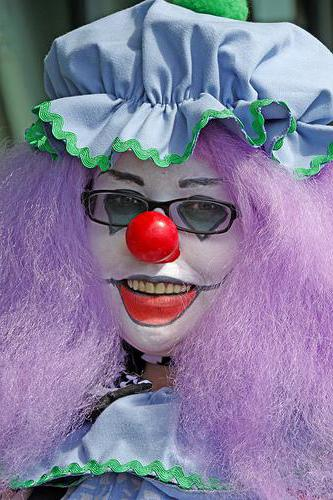
\includegraphics[width=0.2\textwidth]{FLIPPED_fear-394.png}
\caption{The flipped version of the image discussed in the Data section.}
\end{figure}

\begin{figure}
\centering
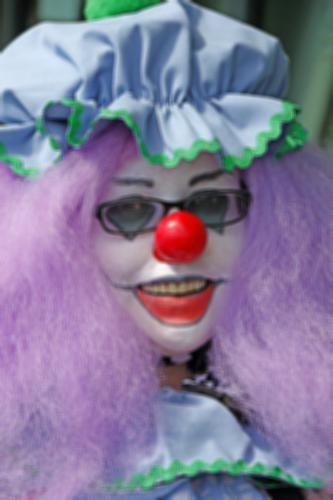
\includegraphics[width=0.2\textwidth]{BLURRED_fear-394.png}
\caption{The blurred version of the same image.}
\end{figure}

\section{Experiment}

Our first step was to evaluate the performance of a simple linear subnetwork tacked on the end of Inception-ResNet. We trained this model with an Adam optimizer and a variety of learning rates to maximize performance on the validation set. (We also tried training with a simple SGD optimizer, and this produced equivalent results, although it required more epochs to train.)

\begin{figure}
\centering
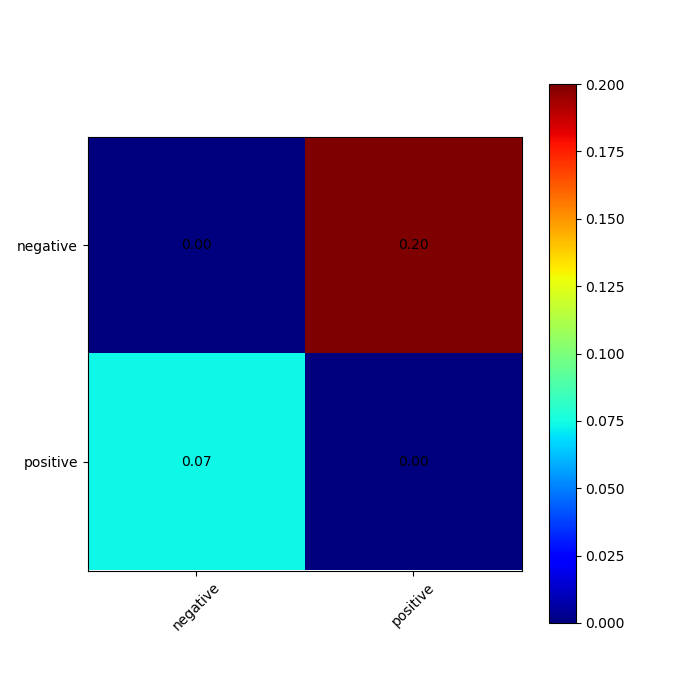
\includegraphics[width=0.5\textwidth]{normalized_confusion_matrix_2_classes_no_hidden.png}
\caption{The confusion matrix for the binary classifier with a linear subnet, if we normalize by the number of examples of each class in the test set.}
\end{figure}

For the binary classification problem, our final accuracy on the test set was 89.5\%. We were curious to see if more of the error came from misclassification of positive or negative valence, since our training data contained more examples of the former. (To be precise, we had 2735 training images for negative valence and 7715 training images for positive valence.) When we normalize by the number of examples belonging to each category in the test set, we discover that we have a 7\% classification error on samples with positive valence, and a 20\% classification error on samples with negative valence. This confirms that our classifier is biased toward samples with positive valence.

\begin{figure}
\centering
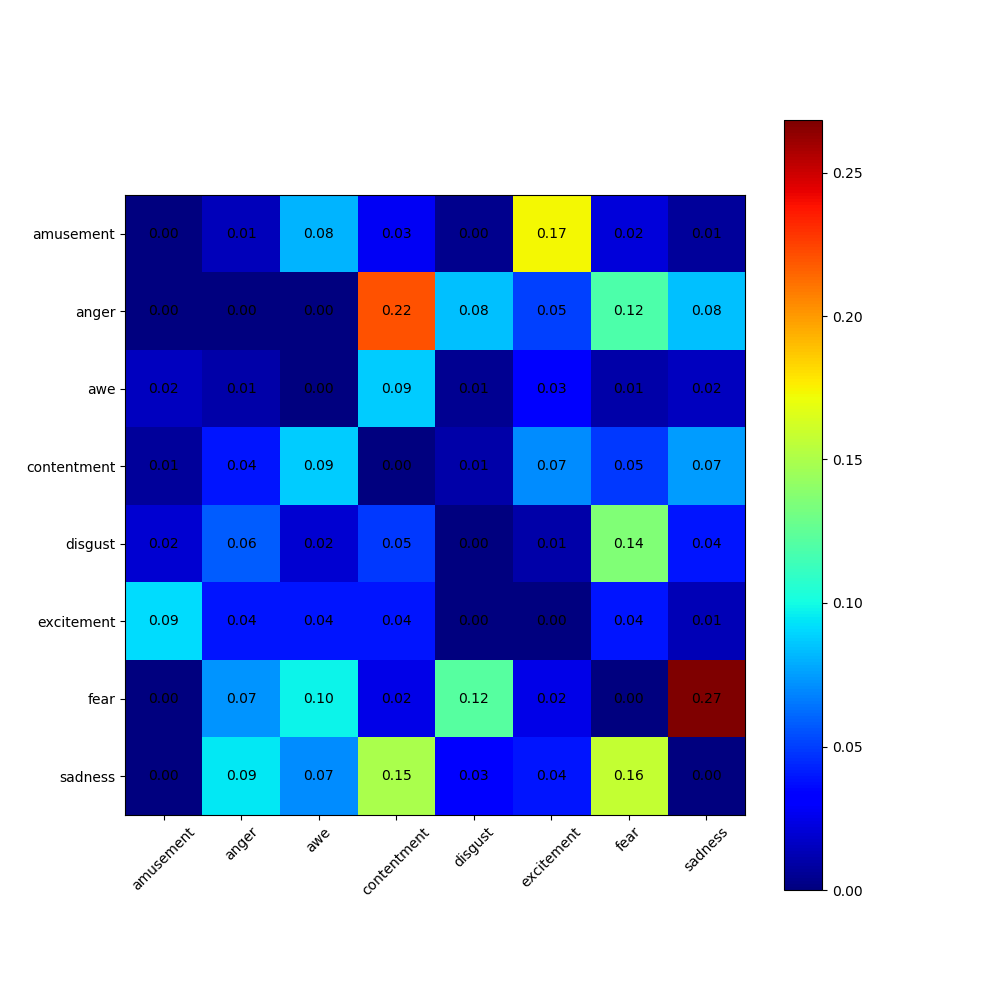
\includegraphics[width=0.5\textwidth]{normalized_confusion_matrix_8_classes_no_hidden.png}
\caption{The confusion matrix for the eight-fold classifier with a linear subnet, normalized by the number of examples belonging to each class in the test set.}
\end{figure}

For the eight-fold classification problem, using a simple linear subnetwork, our final top-1 accuracy on the test set was 66\%. Here, our confusion matrix is worth studying in more detail. We note that our most common misclassification is labeling images of fear as images of sadness. This makes sense, since fear is our smallest class with negative valence and sadness is our largest class with negative valence. If the classifier is able to determine that a picture evoking fear is producing some negative emotion, but is not able to determine which emotion that is, it is likely to guess sadness. However, our second most-common classification error is labeling images of anger as images of contentment. This is less intuitive, since anger and contentment have different valence. Contentment is the largest category in our dataset, whereas anger is one of the smallest. We conclude, then, that there are some images of anger in the test set which the algorithm has no ability to classify, and that it is simply guessing the most probable class a priori.

\begin{figure}
\centering
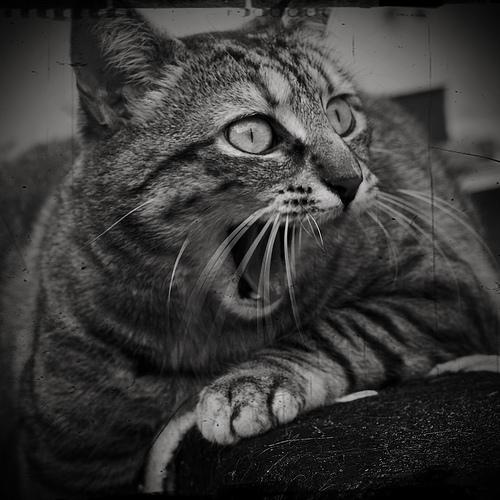
\includegraphics[width=0.3\textwidth]{anger-157.png}
\caption{The truth label for this image is ``anger,'' but the classifier labeled it as ``contentment.'' The best explanation appears to be the fact that ``contentment'' is our largest class, and the algorithm may have encountered nothing similar to this photo in the training data.}
\end{figure}

\begin{figure}
\centering
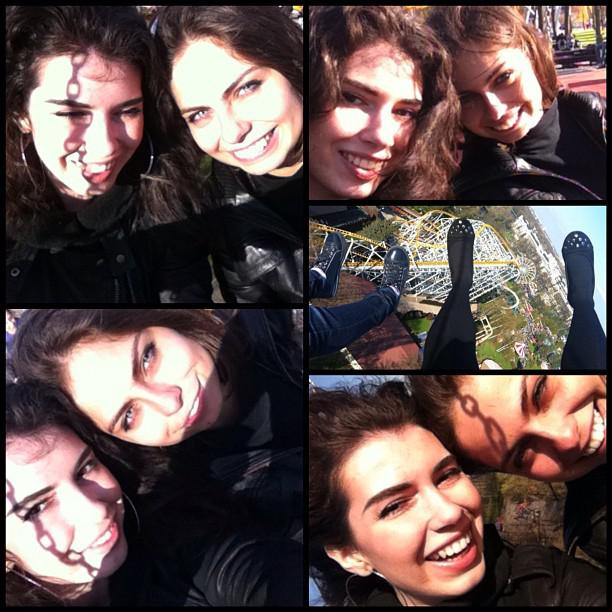
\includegraphics[width=0.3\textwidth]{amusement-12.png}
\caption{The truth label for this image is ``amusement,'' but the classifier labeled it as ``excitement.'' This is a common and intuitive failure case.}
\end{figure}

In addition to the insights above, the confusion matrix suggests that the classifier has high error on two cases:

\begin{enumerate}
  \item \textbf{Images of amusement and excitement are frequently confused with each other.} This matches our intuition that amusement and excitement are similar emotional states. Amusement is rarely confused with contentment, even though contentment also has positive valence and is the largest class in the training set.
  \item \textbf{Images with negative valence are frequently being confused for each other.} It would be nice to conclude, based on this, that images with negative valence are somehow ``more similar'' to each other than images with positive valence, but a more probable explanation is the dearth of training data for these categories. Because our training data was collected through searches on social media platforms, it makes sense that it was easier to gather images with positive valence than images with negative valence--but this bias is reducing our classifier's performance on the smaller classes.
\end{enumerate}

Next, we added a fully-connected hidden layer with 100 units. As explained in the Methods section, we expect that this hidden layer will immediately result in overfitting, since it dramatically increases the size of our parameter space. This was in fact the case. For the binary classification problem, our test accuracy rose from 89\% to 90\%, but our training accuracy rose to 98\%--a clear sign of overfitting. The loss on the validation set also began to increase as we continued training. For the eight-fold problem, our test classification accuracy rose from 66\% to 69\%, but the training classification accuracy rose to 90\%, and once again, the loss on the validation set became worse as training continued. We scanned over several hyperparameter values for L2 regularization, and this ``fixed'' the problem in a way, since it reduced the gap between the training and validation accuracies. The final test accuracy, however, remained constant at 90\% for the binary classifier and 69\% for the eight-fold classifier.

Finally, we decided to try to address our class imbalance problem with image augmentation.

\begin{figure}
\begin{center}
 \begin{tabular}{||c c||} 
 \hline
 Classifier & Accuracy on test set \\ [0.5ex] 
 \hline\hline
 Linear subnet & 66\% \\
 \hline
 One hidden layer & 69\% \\
 \hline
 With regularization & 69\% \\
 \hline
 With image augmentation & ??? \\
 \hline
\end{tabular}
\end{center}
\caption{Eight-fold classification accuracies on the test set for different strategies.}
\end{figure}

\begin{figure}
\begin{center}
 \begin{tabular}{||c c||} 
 \hline
 Classifier & Accuracy on test set \\ [0.5ex] 
 \hline\hline
 Linear subnet & 89\% \\
 \hline
 One hidden layer & 90\% \\
 \hline
 With regularization & 90\% \\
 \hline
 With image augmentation & ??? \\
 \hline
\end{tabular}
\end{center}
\caption{Binary classification accuracies on the test set for different strategies.}
\end{figure}

\section{Conclusion}

In this paper, we tried to determine if transfer learning from ImageNet could produce a classifier which recognized emotion in photos. We gave this classifier two tasks: first, just determine if the photo has negative or positive valence; and second, assign the photo to one of eight emotional categories. The classifier proved to be quite effective at the valence classification problem, but was less effective at the eight-fold classification problem. Our difficulty in training complicated subnets without overfitting suggest that we were hitting the limits of our training data. We may also have been confounded by some of the problems in data collection described in the Data section.

For future work, we suggest that more data needs to be gathered, particularly for the classes with negative valence. The means by which data is gathered also need to be adjusted. Instead of assigning emotions to photos in a one-to-one mapping, it makes more sense to allow humans to assign multiple emotions to a photo. In the case of object recognition, we can argue that there is just one primary object in a photo, and that this should be the label. For emotion recognition, however, it is impossible to ignore the fact that one photo might produce several emotions in an observer. Because these emotions might have different strengths, it would be ideal if the training data assigned a numerical score to the strength of each emotion. Object detection might be a discrete problem--the car is either in the photo, or it is not--but emotion detection is better suited for a regression. Our preliminary results are sufficiently promising that we believe that, if better data were gathered, emotion recognition through computer vision is an achievable goal.

{\small
\bibliographystyle{ieee}
\bibliography{vision_citations}
}


\end{document}
